\documentclass{article}
\usepackage{zref-clever}
\usepackage{enumitem}
\usepackage{graphicx}
\usepackage{float}
\usepackage{hyperref}


\title{Übungszettel 2}
\author{Linus Faber (4764260), Adrian Wünschel (4763715)}

\begin{document}
\maketitle

\begin{abstract}
Dies ist unsere Abgabe zum zweiten Zettel des Moduls Software Engineering (ISE).
Unser Verlauf ist einsehbar unter unserem \href{https://github.com/LinusFaber/ise26-27_assignment02}{Repository}.
\end{abstract}

\section*{Aufgabe 2.1}
\label{sec:a21}

\begin{enumerate}[label=\alph*)]

  \item % a)
  \begin{itemize}
    \item Kotlin:
    \begin{itemize}
      \item \texttt{:build}
      \item \texttt{:check}
      \item \texttt{:assemble}
    \end{itemize}
    \item Application:
    \begin{itemize}
      \item \texttt{:distZip}
      \item \texttt{:distTar}
      \item \texttt{:startScripts}
    \end{itemize}
    \item ktlint:
    \begin{itemize}
      \item \texttt{:loadKtlintReporters}
      \item \texttt{:runKtlintCheckOverKotlinScripts}
      \item \texttt{:ktlintKotlinScriptCheck}
      \item \texttt{:runKtlintCheckOverMainSourceSet}
      \item \texttt{:ktlintMainSourceSetCheck}
      \item \texttt{:runKtlintCheckOverTestSourceSet}
      \item \texttt{:ktlintTestSourceSetCheck}
    \end{itemize}
    \item detekt:
    \begin{itemize}
      \item \texttt{:detekt}
    \end{itemize}
  \end{itemize}

  Für \texttt{:distTar} und \texttt{:startScripts} haben wir uns von Gemini helfen lassen.

  \item % b)
  3 failures:

  \begin{itemize}
    \item \texttt{:detekt}, \texttt{DoublyLinkedList.kt:98}, MagicNumber
    \item \texttt{ktlintMainSourceSetCheck}, \texttt{DoublyLinkedList.kt:98:}, Missing spacing after "if"
    \item \texttt{:test}, \texttt{DoublyLinkedList.kt:101}, NullPointerException
  \end{itemize}

  \texttt{-{-}continue} führt auch noch die weiteren Tasks nach einem Error aus.

  \item % c)
  gradle check macht exklusiv \texttt{:detekt} und \texttt{:ktlintMainSourceSetCheck}.

  Dann macht gradle test diese nicht, \texttt{:test} aber schon und bekommt auch nur dort den Failure.
\end{enumerate}

\section*{Aufgabe 2.2}
\label{sec:a22}

\begin{enumerate}[label=\alph*)]

  \item % a)
  -
  \item % b)
  Nach der Änderung sind alle Tests successful.

  \texttt{DoublyLinkedListTest > testGetThrowsForInvalidIndex() PASSED}

  \texttt{DoublyLinkedListTest > testGetReturnsValueAtIndex() PASSED}

  \item %c)
  BUILD SUCCESSFUL in 1s

  12 actionable tasks: 6 executed, 6 up-to-date

  Configuration cache entry reused.

  \item % d)
  Es wurde kein Workflow Lauf gestartet, weil in dem on-Abschnitt nur main als Branch genannt wird.

  \item % e)
  Screenshot:

  \begin{figure}[H]
    \centering
    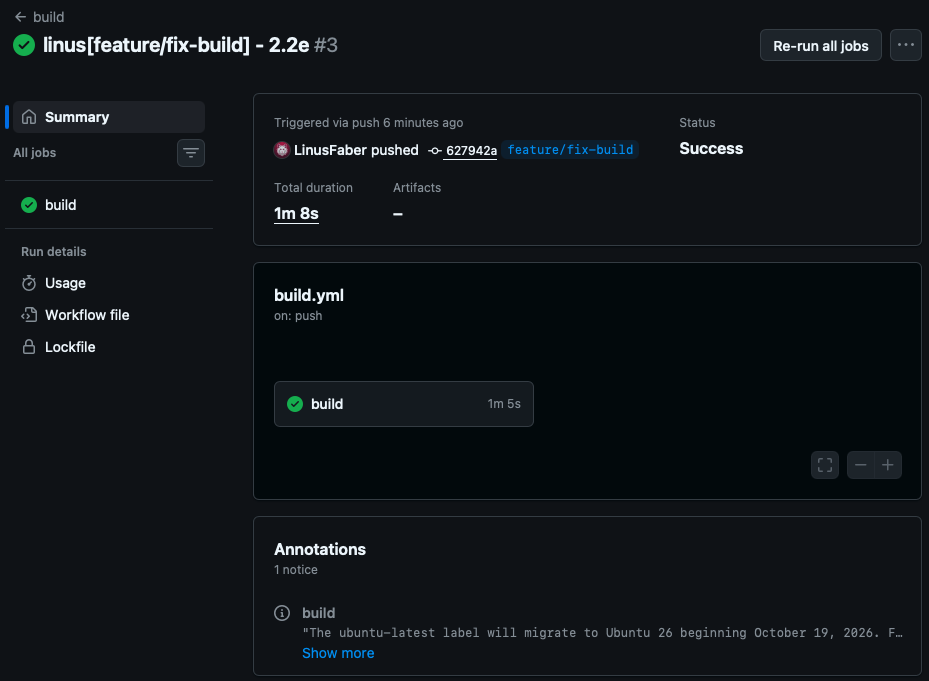
\includegraphics[width=0.8\textwidth]{pics/push_build.png}
    \caption{Push Build}
    \label{fig:push_build}
  \end{figure}

  \newpage

  \item % f)
  Screenshot:

  \begin{figure}[H]
    \centering
    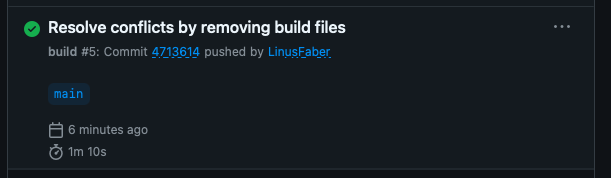
\includegraphics[width=0.8\textwidth]{pics/resolve.png}
    \caption{Resolve}
    \label{fig:resolve}
  \end{figure}

\end{enumerate}


\section*{Aufgabe 2.3}
\label{sec:a23}

\begin{enumerate}[label=\alph*)]
  \item % a)
  Befehl um Datei ausführen zu können:

  \texttt{chmod +x .git/hooks/pre-commit}

  \item % b)
  \texttt{Task :ktlintMainSourceSetCheck FAILED}

  after Fix:

  BUILD SUCCESSFUL in 1s

  7 actionable tasks: 2 executed, 5 up-to-date

  Configuration cache entry reused.

  [main 909e2fb] linus[main] - a2.3b hooktesting after ktlintFormat

  \item % c)
  Warum führt die CI-Pipeline die Checks trotzdem aus?

  \begin{itemize}
    \item   Hooks laufen lokal und können übersprungen werden.
    \item Wir wissen und finden keinen zweiten Grund. Bitte um Rückmeldung welcher?!
  \end{itemize}

\end{enumerate}

\end{document}
